\section{Evaluating Progress}
\subsection{}

\begin{frame}
    \frametitle{Sprint Progress}
    \begin{itemize}
        \setlength\itemsep{0.7em}
        \item At any point in time in a Sprint, the total work remaining in the Sprint Backlog can be summed
        \item The Development Team tracks this total work remaining at least for every \textbf{Daily Scrum}
        \item It then evaluates the likelihood of achieving the Sprint Goal
    \end{itemize}
\end{frame}

\begin{frame}
    \frametitle{Release Progress}
    \begin{columns}
        \begin{column}{0.5\textwidth}
            \begin{itemize}
                \setlength\itemsep{0.7em}
                \item At any point in time, the total work remaining to reach a goal can be summed
                \item The Product Owner tracks this total work remaining at least every \textbf{Sprint Review}
                \item Compares this amount with work remaining at previous Sprint Reviews to assess progress toward completing projected work
            \end{itemize}
        \end{column}
        \begin{column}{0.5\textwidth}
            \vspace{-1em}
            \begin{figure}
                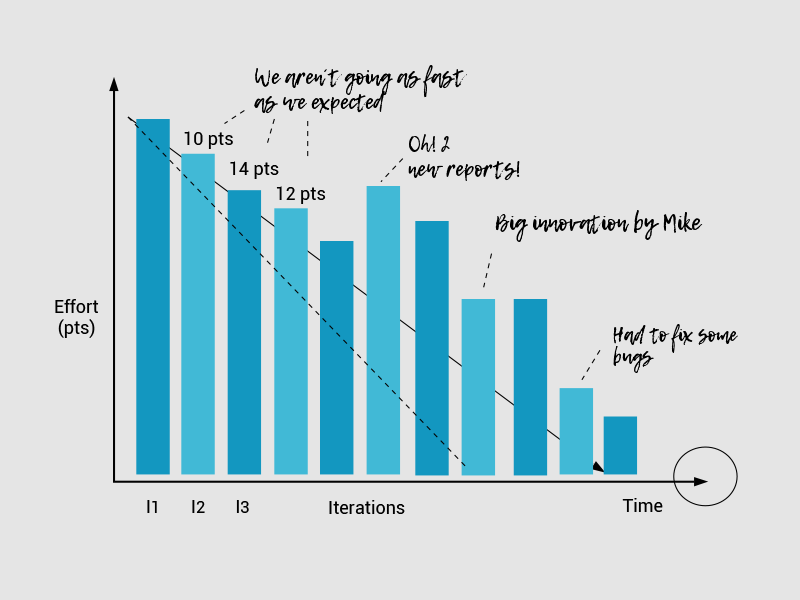
\includegraphics[width=2.7in]{images/burndown.png}
            \end{figure}
        \end{column}
    \end{columns}
\end{frame}